\newcommand{\mcc}[1]{\makebox[6em][c]{#1}}

\newcommand{\jitterof}[2]{\sigma^2_{#1,#2}}
\newcommand{\jitterij}{\jitterof{i}{j}}

\newcommand{\oneminusd}{1\!-\!d}
\newcommand{\nref}{{N_r}}
\newcommand{\ntest}{{N_t}}
\newcommand{\nunder}{{N_u}}

\newcommand{\fgbgonedfig}{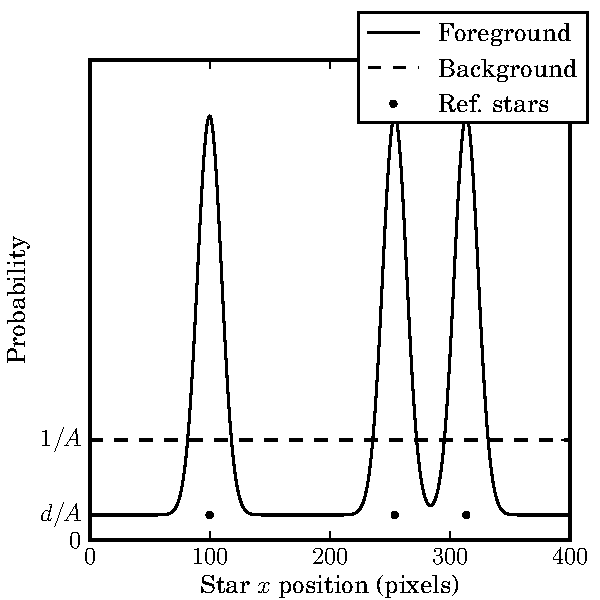
\includegraphics[width=1.000000\figunit]{fgbg-1d}}
\newcommand{\fgbgtwodfig}{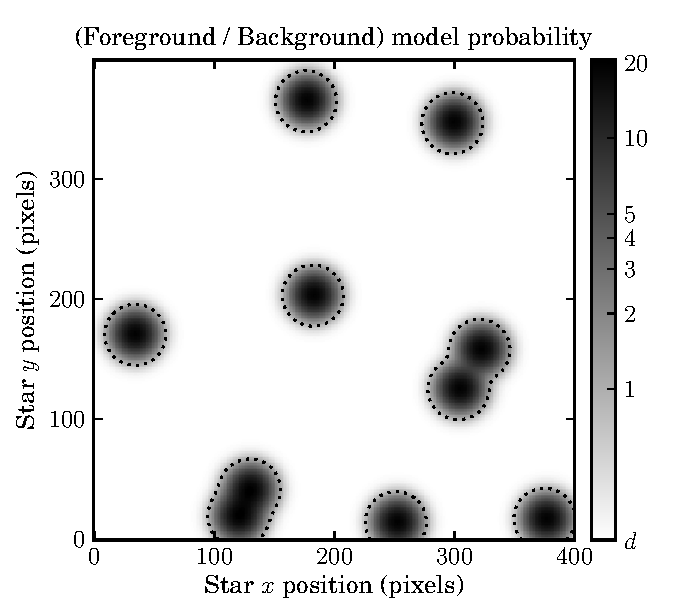
\includegraphics[width=1.150000\figunit]{fgbg-2d}}\newcommand{\symmbgfig}{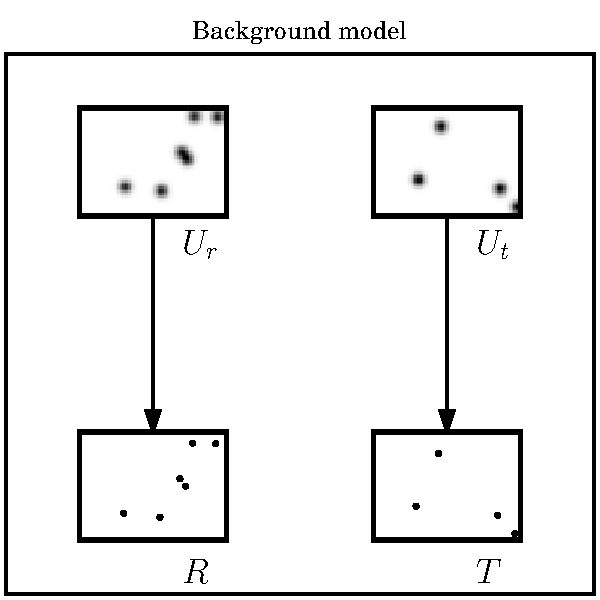
\includegraphics[width=1.000000\figunit]{symm-bg}}
\newcommand{\symmfgfig}{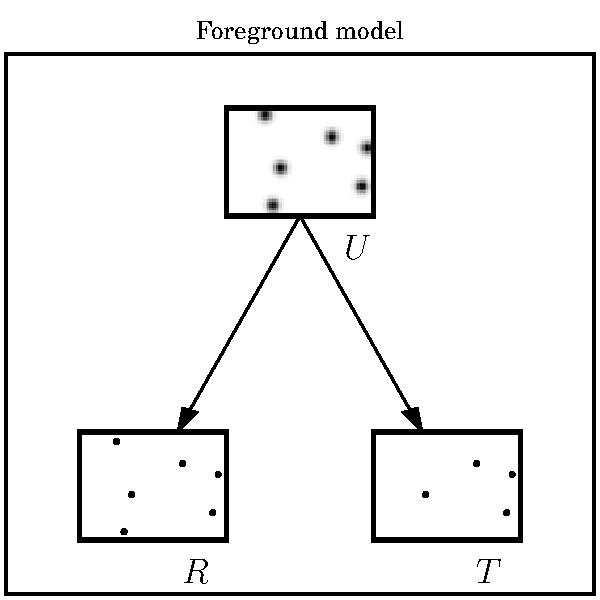
\includegraphics[width=1.000000\figunit]{symm-fg}}\newcommand{\gcreffig}{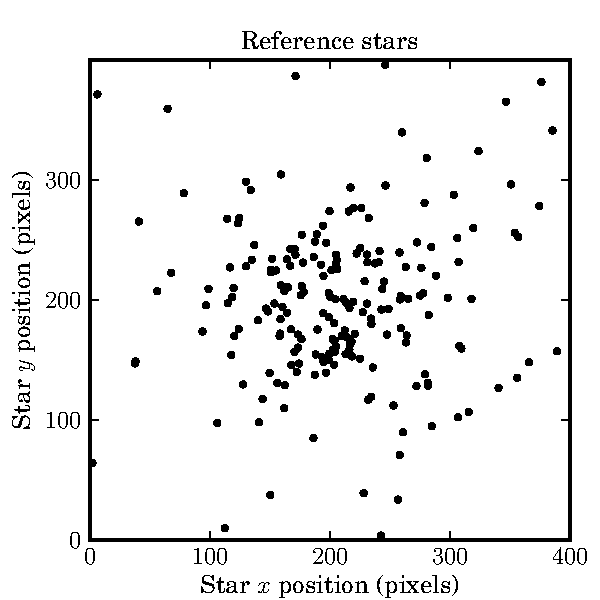
\includegraphics[width=1.000000\figunit]{gc-ref}}
\newcommand{\gctestfalsefig}{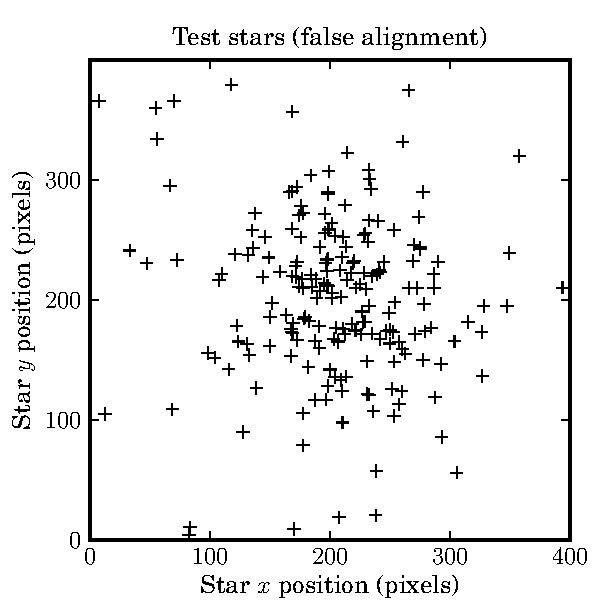
\includegraphics[width=1.000000\figunit]{gc-test-false}}
\newcommand{\gctesttruefig}{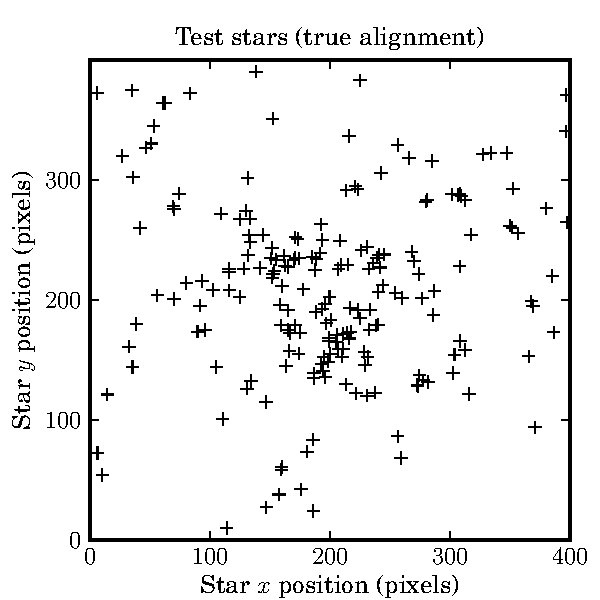
\includegraphics[width=1.000000\figunit]{gc-test-true}}
\newcommand{\gcterrainonefig}{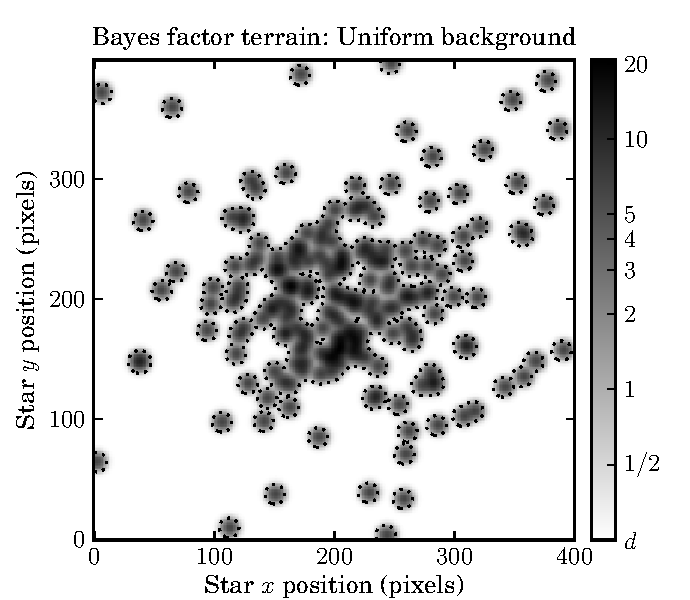
\includegraphics[width=1.150000\figunit]{gc-odds-false1}}
\newcommand{\gcterraintwofig}{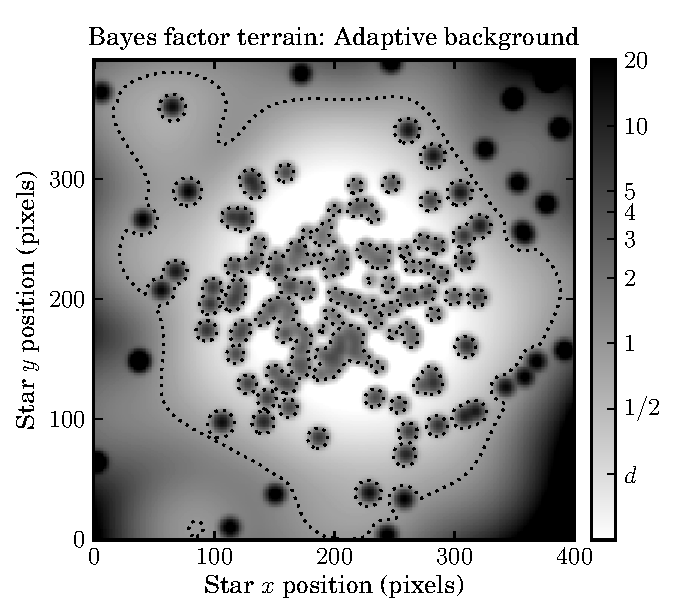
\includegraphics[width=1.150000\figunit]{gc-odds-false2}}
\newcommand{\gcbgtwofig}{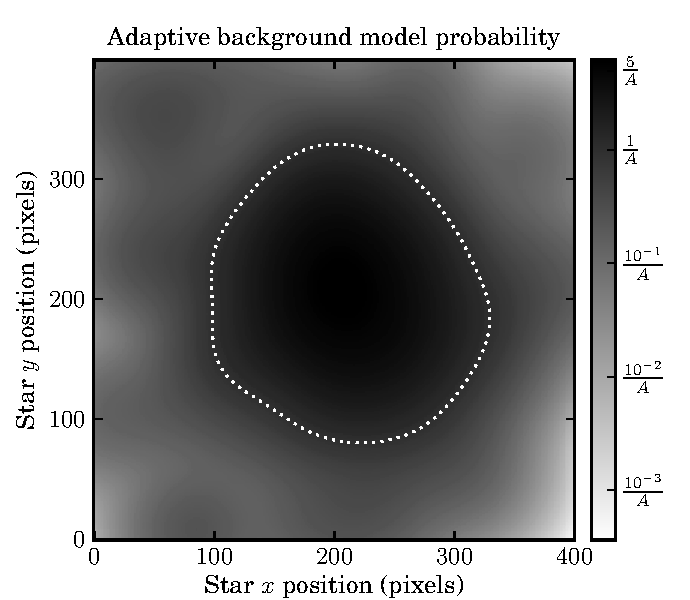
\includegraphics[width=1.150000\figunit]{gc-odds-bg}}
\newcommand{\gcbayesonefig}{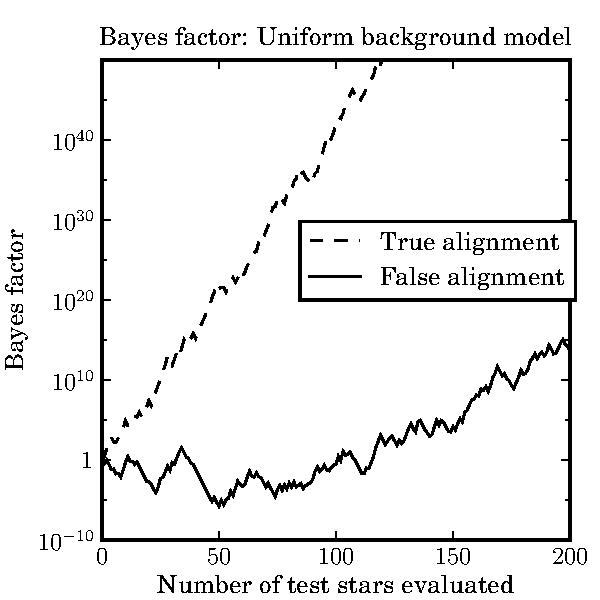
\includegraphics[width=1.000000\figunit]{gc-bayes1}}
\newcommand{\gcbayestwofig}{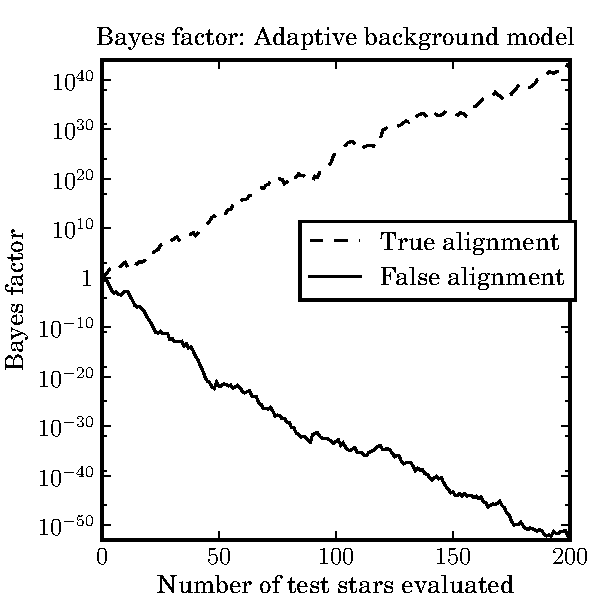
\includegraphics[width=1.000000\figunit]{gc-bayes2}}\newcommand{\nstarsfgone}{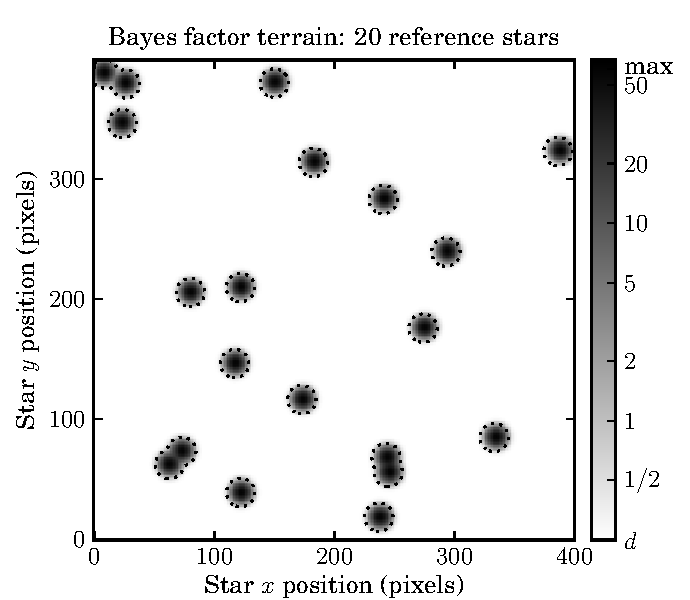
\includegraphics[width=1.150000\figunit]{nstars-fg1}}
\newcommand{\nstarsfgtwo}{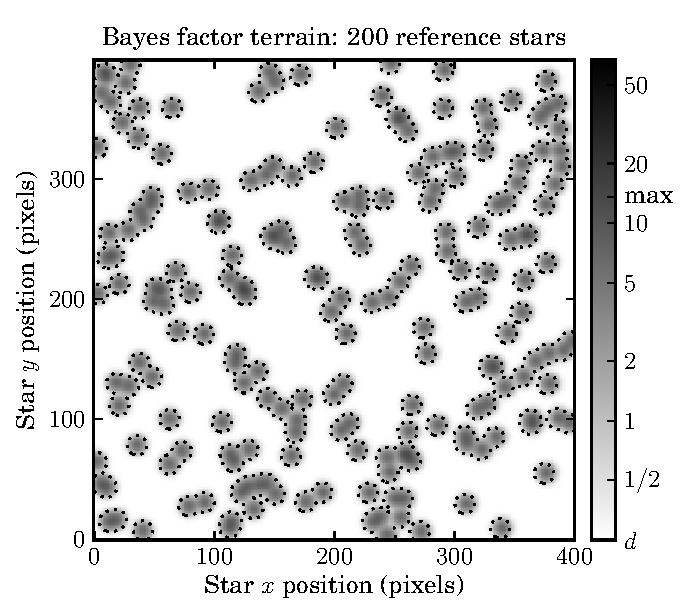
\includegraphics[width=1.150000\figunit]{nstars-fg2}}
\newcommand{\nstarsbayes}{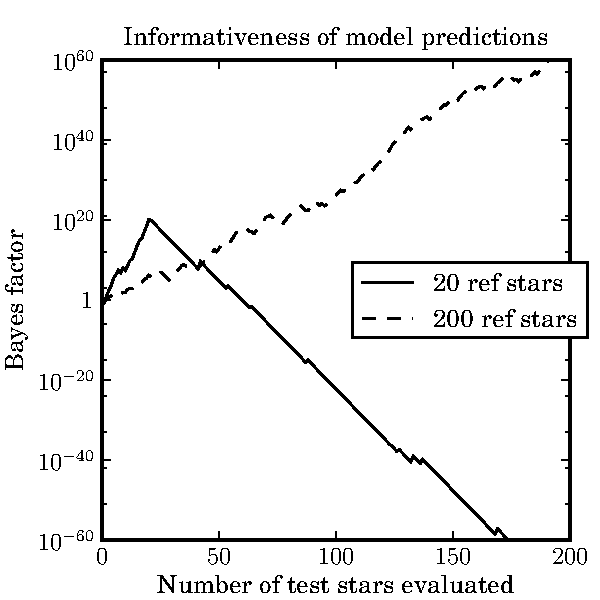
\includegraphics[width=1.000000\figunit]{nstars-bayes}}\newcommand{\exgainareafig}{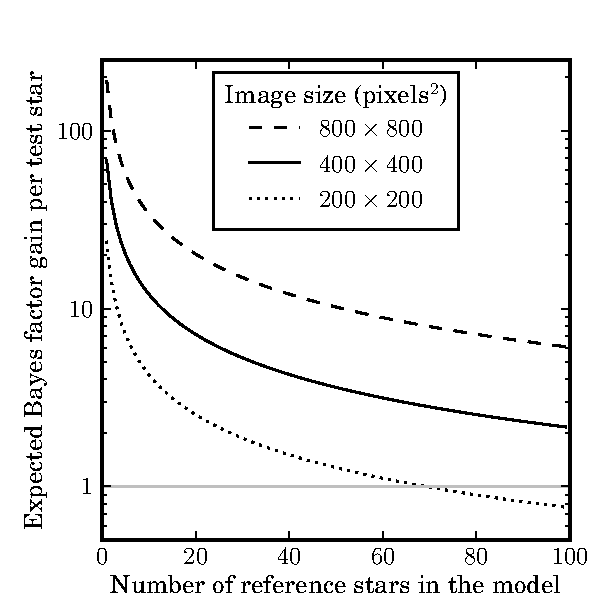
\includegraphics[width=1.000000\figunit]{exgain-1}}
\newcommand{\exgaindfig}{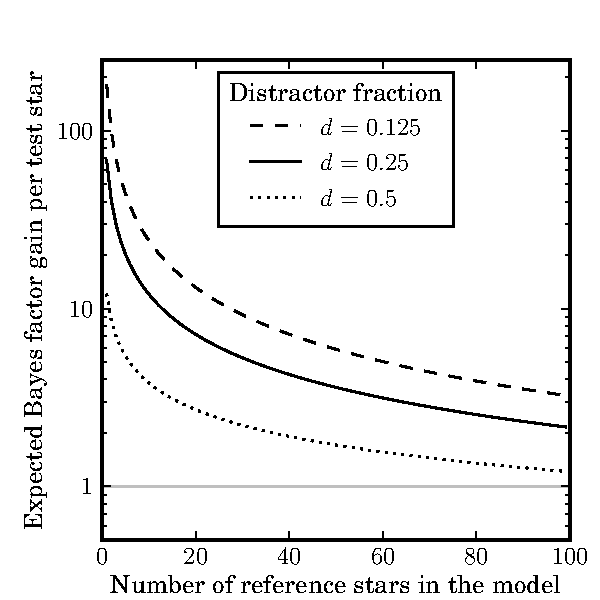
\includegraphics[width=1.000000\figunit]{exgain-2}}
\newcommand{\exgaintotalareafig}{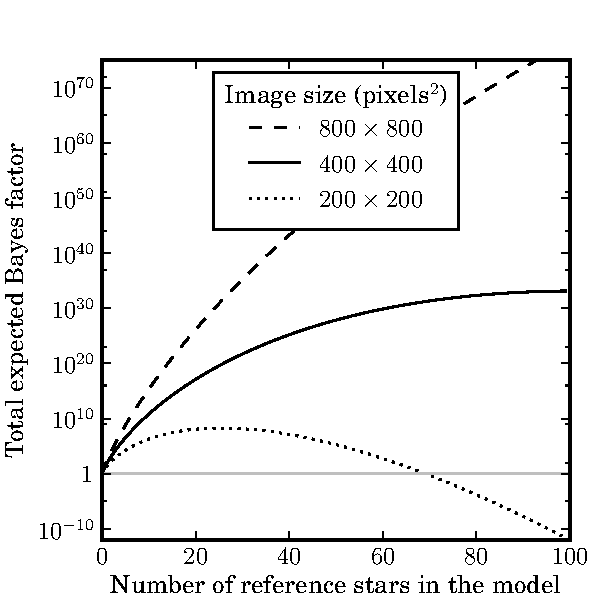
\includegraphics[width=1.000000\figunit]{exgain-total-1}}
\newcommand{\exgaintotaldfig}{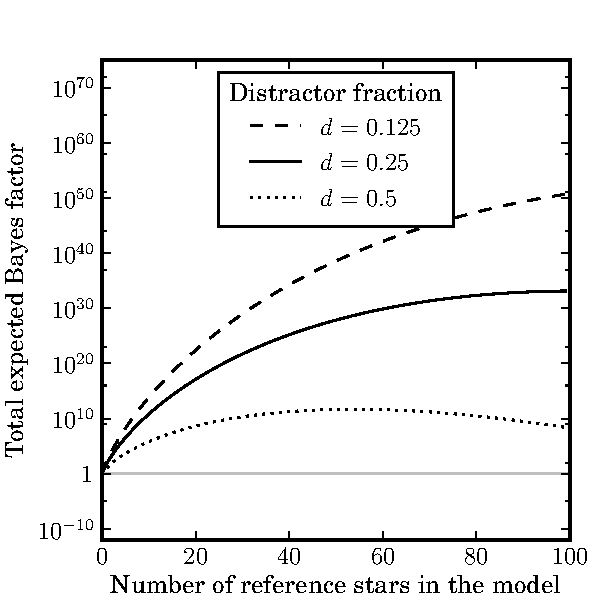
\includegraphics[width=1.000000\figunit]{exgain-total-2}}\newcommand{\donutreffig}{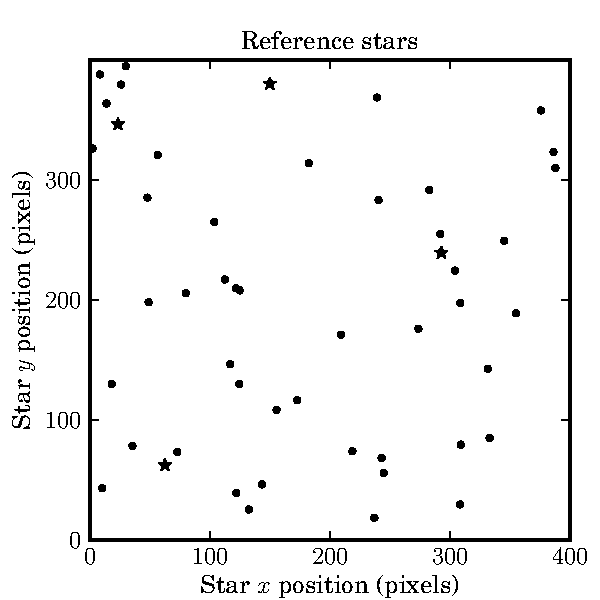
\includegraphics[width=1.000000\figunit]{donut-ref}}
\newcommand{\donuttestfig}{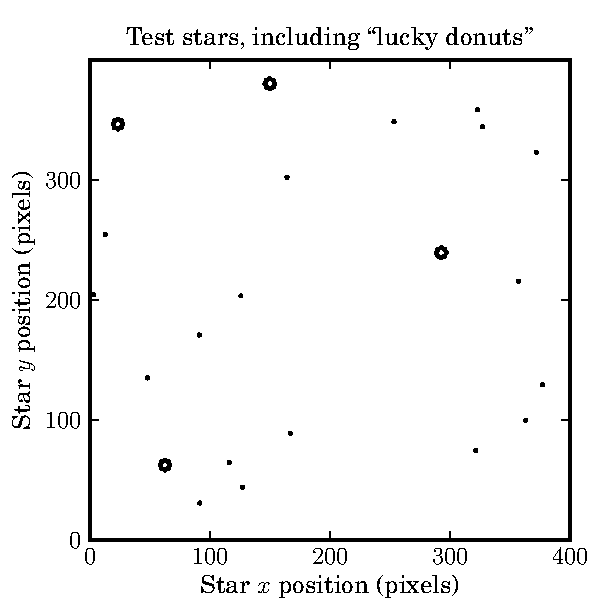
\includegraphics[width=1.000000\figunit]{donut-test}}
\newcommand{\donutbayesfig}{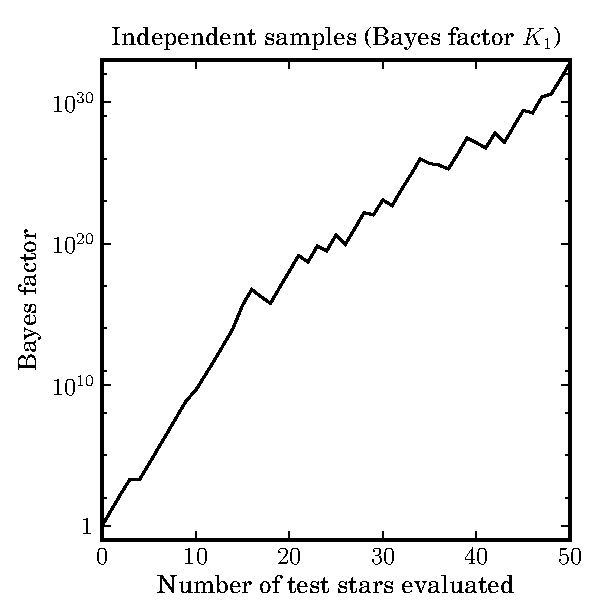
\includegraphics[width=1.000000\figunit]{donut-bayes}}
\newcommand{\donutthetasfig}{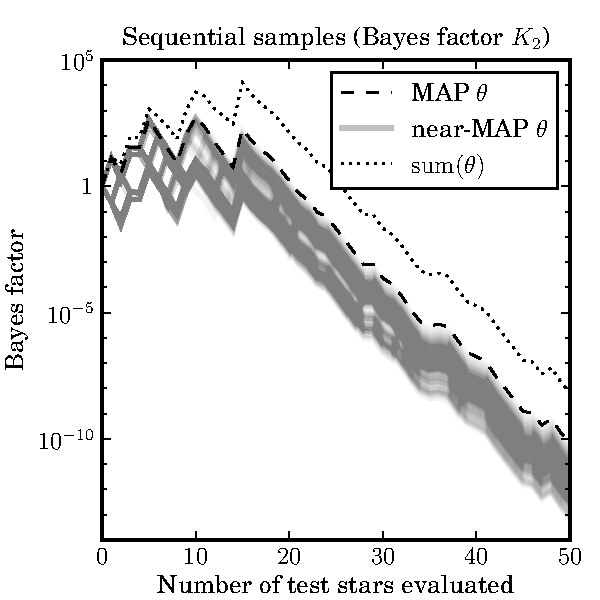
\includegraphics[width=1.000000\figunit]{donut-thetas}}\newcommand{\rorrotationfig}{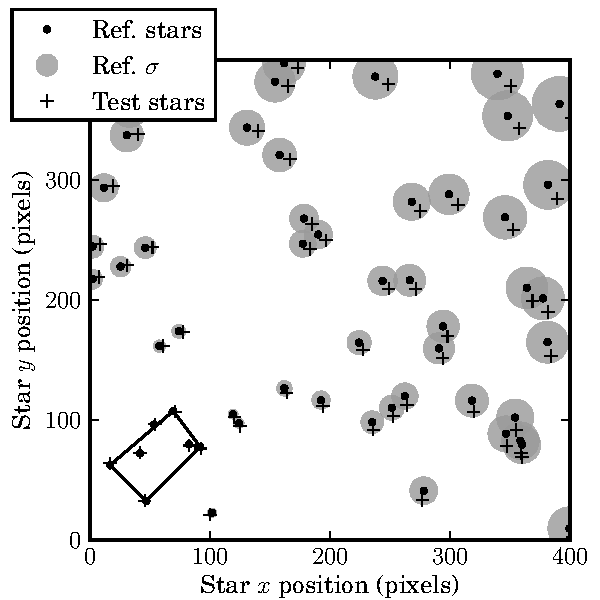
\includegraphics[width=1.000000\figunit]{ror-rotation}}
\newcommand{\rorbayesfig}{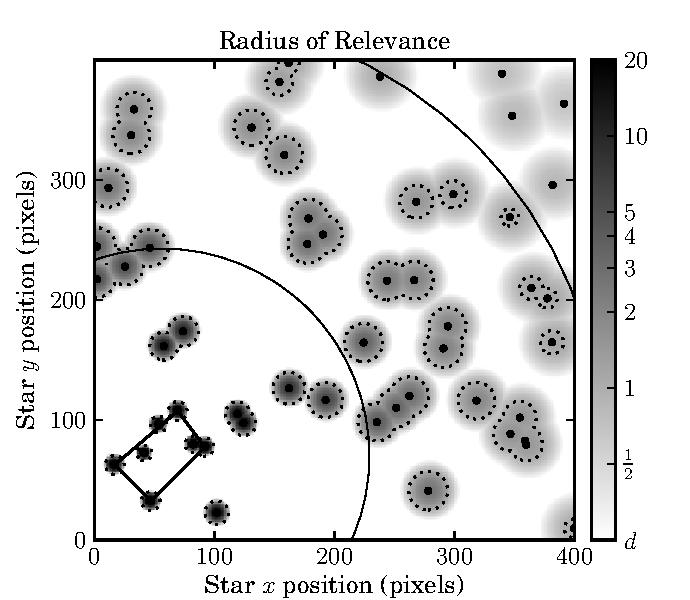
\includegraphics[width=1.150000\figunit]{ror-bayes}}


%\begin{abstract}
%Abstract.
%\end{abstract}

% Astro-intro:
%  --decisions are sometimes easier than inference!

\section{Introduction}


Suppose we are given two lists of astronomical sources (``stars'',
hereafter) and a hypothesized astrometric alignment between them.  We
wish to produce a probabilistic assessment of whether the alignment is
true or false, where a false alignment might nonetheless show some
coincidentally matching stars.  For example, one list might be an
astrometric reference catalog and the other a list of stars detected
in an image, and the hypothesized alignment could be a World
Coordinate System (WCS) transformation that maps pixel coordinates in
the image to celestial coordinates in the reference catalog.  We then
wish to assess whether applying the given transformation to the stars
detected in the image causes them to align with the stars in the
reference catalog.


We assume that the lists of stars include the positions, positional
uncertainties, and an approximate brightness ordering.  We assume that
the positional errors are drawn from known probability distributions
that are correctly described by the positional uncertainties.  In this
\doctype we will assume the positional errors are drawn from Gaussian
distributions whose variances are given by the positional
uncertainties.


In true alignments, some fraction of the stars in each list will have
no counterpart in the other list.  This could be due to occlusions in
the images (from which the lists of stars are produced), artifacts or
errors in detecting stars, or differences in the spectral bandpass or
sensitivity of the two images.  True stars can be missing from, and
false stars added to, either list.  The lists may be of quite
different lengths due to different sensitivities and error rates.


\comment{
  We assume that the true stars that appear in both lists will generally
  be assigned the same relative brightness ordering.  This is roughly
  equivalent to assuming that the spectral bandpasses are similar.
}

\comment{
  ---why this very soft assumption about ordering rather than a stronger
  assumption involving brightness in different bands, errors in measured
  brightness, etc.
  }

\comment{
  ---desiderata: robustness given distractors/dropouts: simplicity;
  efficiency (speed); sensitivity; conservativeness (in avoiding
  false positives)
  }

Since our goal is to decide whether to accept or reject a proposed
alignment, and we assume a probabilistic model, we can frame the
problem in terms of Bayesian decision theory.  This is briefly
reviewed in the following section.  We then proceed in
\secref{sec:simple} to develop a simple model, point out the ways in
which it fails and modify the model to handle these concerns.  This
problem is central to the \an system, which uses geometric hashing to
generate a large number of hypotheses which must be checked.  We
explore the specifics of the \an application in
\secref{sec:an}.


\section{Bayesian decision-making}


We wish to decide whether to accept or reject a proposed alignment.
In effect, we are choosing between two models: a ``foreground'' model,
in which the alignment is true, and a ``background'' model, in which
the alignment is false.  In Bayesian decision-making, three factors
contribute to this decision: the relative abilities of the models to
explain the observations, the relative proportions of true and false
alignments we expect to see, and the relative costs or utilities of
the outcomes resulting from our decision.


The \emph{Bayes factor} $K$ is a quantitative assessment of the
relative abilities of the two models---the foreground model $\fg$ and
the background model $\bg$---to produce or explain the observations.  In
this case the observations, or data, $\data$, are the two lists of stars.
The Bayes factor
\begin{equation}
K = \frac{p(\data \given \fg)}{p(\data \given \bg)}
\label{eq:bayesf}
\end{equation}
is the ratio of the marginal likelihoods.  We must also include in our
decision-making the prior $p(\fg)/p(\bg)$, which is our \emph{a priori}
belief, expressed as a ratio of probabilities, that a proposed
alignment is correct.  In the \an case, for example, we typically
examine many more false alignments than true alignments, so this ratio
will be small.

The final component of Bayesian decision theory is the \emph{utility}
table, which expresses the subjective value of each outcome.  In this
problem, there are four possible outcomes: If the alignment we are
considering is true and we decide to accept it, the outcome is a true
positive (``\truepos''), while if we reject it we generate a false
negative (``\falseneg'').  If the alignment is false and we accept it,
we produce a false positive outcome (``\falsepos''), while if we
reject it we get a true negative (``\trueneg'').  The utility table,
as shown below, assigns a value $u(\cdot)$ to each of these outcomes.

\nonumberparagraphs
\begin{center}
\begin{tabular}{|c|c|c@{\extracolsep{\fill}}|c|}
  \cline{3-4}
  \multicolumn{2}{c|}{} & \multicolumn{2}{c|}{True Alignment? \tstrut} \\
  \cline{3-4}
  \multicolumn{2}{c|}{} & \multicolumn{1}{c|}{\mcc{Yes}} & \mcc{No \tstrut} \\
  \hline
  \multirow{2}{*}{Decision} & Accept & \mcc{$u(\truepos)$} & \mcc{$u(\falsepos)$ \tstrut} \\
  \cline{2-4}
  & Reject & \mcc{$u(\falseneg)$} & \mcc{$u(\trueneg)$ \tstrut} \\
  \hline
\end{tabular}
\end{center}
\numberparagraphs


We make our decision to accept or reject the proposal by computing the
expected utility $\expect{u}$ of each decision.  The expected utility
of accepting the alignment is:
\begin{align}
\expect{u \given \mathrm{Accept}, \data}
&= u(\truepos) \, p(\truepos \given \data) + u(\falsepos) \, p(\falsepos \given \data) \\
&= u(\truepos) \, p(\fg \given \data) + u(\falsepos) \, p(\bg \given \data)
\end{align}
while the expected utility of rejecting the alignment is:
\begin{align}
\expect{u \given \mathrm{Reject}, \data}
&= u(\falseneg) \, p(\falseneg \given \data) + u(\trueneg) \, p(\trueneg \given \data) \\
&= u(\falseneg) \, p(\fg \given \data) + u(\trueneg) \, p(\bg \given \data) \quad .
\end{align}
We should accept the hypothesized alignment if:
\begin{align}
\expect{u \given \mathrm{Accept}, \data} 
&>
\expect{u \given \mathrm{Reject}, \data} \\
%
u(\truepos) \, p(\fg \given \data) + u(\falsepos) \, p(\bg \given \data)
&>
u(\falseneg) \, p(\fg \given \data) + u(\trueneg) \, p(\bg \given \data) \\
%
%\big( u(\truepos) - u(\falseneg) \big) \  \frac{p(\fg \given \data)}{p(\bg \given \data)}
%&>
%u(\trueneg) - u(\falsepos) \\
%
\frac{p(\fg \given \data)}{p(\bg \given \data)}
&>
\frac{u(\trueneg) - u(\falsepos)}{u(\truepos) - u(\falseneg)} \\
%
K &> \frac{p(\bg)}{p(\fg)} \ \frac{u(\trueneg) - u(\falsepos)}{u(\truepos) - u(\falseneg)}
\label{eq:kthresh}
\end{align}
where we have applied Bayes' theorem to get
\begin{equation}
\frac{p(\fg \given \data)}{p(\bg \given \data)} = K \ \frac{p(\fg)}{p(\bg)} \quad .
\end{equation}


That is, we accept or reject a proposed alignment by thresholding the
Bayes factor of the foreground model to the background model.  The
threshold is set based on our desired operating point for the
particular application.  Increasing the threshold will cause us to
reject more proposals, thus changing some false positives to true
negatives (increasing the utility), while changing some true positives
to false negatives (decreasing the utility).


There is an arbitrary overall scaling of the utility values, since in
\eqnref{eq:kthresh} only the ratios of differences of utilities
appear.  When setting utility values, it may be convenient to set
$u(\truepos) = 1$ and choose the other utilities relative to that.  In
that case, the $u(\falsepos)$ and $u(\falseneg)$ values may be
negative.  In the \an case, for example, we want strongly to avoid
false positives, so the ratio of utility differences is dominated by
$u(\falsepos) \ll 0$, and combined with the small prior
$p(\fg)/p(\bg)$ mentioned earlier, we find that $K$ must be very
large: we demand that the foreground model be an overwhelmingly better
explanation of the data before accepting the hypothesis.


\section{A simple independence model}
\label{sec:simple}


In this section we consider one of the lists to be a fixed
``reference'' list, and develop foreground and background models in
which each star in the other ``test'' list is treated as an
independent sample from the model.  In this case, the Bayes factor
(\eqnref{eq:bayesf}) becomes:
\begin{equation}
  K_1 = \frac{p(\data \given \fg)}{p(\data \given \bg)} = \prod_{i=1}^\ntest \frac{p(t_i \given \fg)}{p(t_i \given \bg)}
  \label{eq:K1}
\end{equation}
where $t_i$ is the $i$th star in the test list, and the reference list
is used to define the foreground model.  We have added the subscript
$K_1$ to identify this definition of the Bayes factor: we will use
different definitions in later sections.


%\subsection{Foreground model}

\begin{figure}
\begin{center}
\begin{tabular}{@{}c@{}c@{}}
\fgbgonedfig &
\fgbgtwodfig \\
\end{tabular}
\end{center}
\caption{\captionpart{Left:} one-dimensional slice of the simple
  foreground and background probability distributions $\fgone$ and
  $\bgone$.  The background model is uniform, while the foreground
  model has a uniform floor plus Gaussian peaks around each reference
  star.  \captionpart{Right:} two-dimensional probability density
  ratio of the foreground to background models---the Bayes factor
  terrain for a single test star---on a log scale.  The contours
  indicate where the models are equal.  In these plots, the distractor
  fraction $d = 0.25$, $\jitterij = 10$, and the image size is $400
  \times 400$ pixels.  This value of $\jitterij$ is larger than is
  typical in astronomical images in order to make the figures more
  clear.
  \label{fig:fgbg}}
\end{figure}

In the foreground model, each test star is generated either by a
reference star, or by an object that does not appear in the reference
list: possibly a real star, possibly an artifact.  If a test star is
generated by a reference star, then its observed position is
distributed according to the positional variances of the reference and
test stars.  If a test star is not generated by a reference star, we
assume it will be observed with uniform probability anywhere in the
image.  We call test stars that are not generated by reference stars
``distractors.''  Distractor stars can be generated if the test star
corresponds to a real star that does not appear in the reference list,
or if the test star is actually an artificial satellite, a planet, a
cosmic ray, a false positive in the star detection process, or some
other kind of artifact.  The distractor component of the model is a
catch-all for artifacts and errors in both the test and reference
lists.  In general we expect stars to be both added and removed from
both lists, but since it is difficult to determine whether a
distractor is due to a star being added to the test list or removed
from the reference list, we lump these cases together.


This foreground probability model, $\fgone$, is thus a mixture of a
uniform distribution of distractor stars, plus a Gaussian distribution
around each reference star:
\begin{equation}
  p(t_i \given \fgone) = \frac{d}{A} + \frac{\oneminusd}{\nref} \sum_{j=1}^{\nref} \pgauss{t_i}{r_j}{\jitterij}
  \label{eq:pf1}
\end{equation}
where $d$ is the fraction of distractor stars, $A$ is the area of the
image, and $\{r_j\}$ are the $\nref$ reference stars.
$\pgauss{x}{\mu}{\sigma^2}$ is the probability of drawing value $x$
from the Gaussian distribution with mean $\mu$ and variance
$\sigma^2$.  Note that $t_i$ and $r_j$ are both two-dimensional
vectors (positions in the image plane).  We have written the combined
positional variance of test star $i$ and reference star $j$ \mbox{as
$\jitterij$.}


%\subsection{Background model}

In the background model, test stars are drawn without regard for the
positions of the reference stars.  The simplest model, $\bgone$, is
that the test stars are distributed uniformly across the image:
\begin{equation}
  p(t_i \given \bgone) = \frac{1}{A}
  \label{eq:pb1}
\end{equation}
where, as before, $A$ is the area of the image.  These models are
illustrated in \figref{fig:fgbg}.


Observe that the background model probability density sums to unity
over the area of the image, while the foreground model yields a value
very slightly less than unity since the Gaussians around each
reference star have infinite support but the image is finite.  Since
the positional variances in typical astronomical images are small
relative to the image size, this effect is negligible.


\subsection{Issues with this model}


We will now present a number of different problems with this simple
setting, adjusting the models to address each concern.  Some of the
scenarios we describe may seem contrived, but in \an we have
encountered most of them in real data.


\subsubsection{Asymmetric model structure}
\label{sec:symm}

\begin{figure}
\begin{center}
\begin{tabular}{@{}c@{}c@{}}
\symmbgfig &
\symmfgfig \\
\end{tabular}
\end{center}
\caption{Left: ``background'' model: the reference star list $R$ and
  test star list $T$ are unrelated: each is generated by sampling from
  its own underlying probability density of stars ($U_r$ and $U_t$,
  respectively).  Right: ``foreground'' model: star lists $R$ and $T$
  are two samples from a common underlying probability distribution of
  stars, $U$.
\label{fig:symm}}
\end{figure}



One might ask why we have chosen a setting that treats reference and
test stars differently, as opposed to a setting such as that pictured
in \figref{fig:symm}, in which reference and test stars are treated
symmetrically.  Instead of asking whether the reference stars predict
the test stars, we could select between two models: in the background
model, the reference and test lists are derived from independent
underlying lists (\ie, they are images of different parts of the sky),
while in the foreground model they are derived from a single shared
list (\ie, they are images of the same part of the sky).


In this symmetric setting, the foreground and background model
probabilities become
\begin{align}
  p(\data \given \fgsymm) &=
  \int
  \prod_{i=1}^{\ntest} p(t_i \given U, \fgsymm)
  \prod_{j=1}^{\nref} p(r_j \given U, \fgsymm)
  \ p(U)\  \dd U \\
  %
  p(\data \given \bgsymm) &=
  \int
  \prod_{i=1}^{\ntest} p(t_i \given U_t, \bgsymm)
  \ p(U_t) \ \dd U_t
  \int
  \prod_{j=1}^{\nref} p(r_j \given U_r, \bgsymm)
  \ p(U_r) \ \dd U_r
\end{align}
where we must marginalize over the shared parameters $U$ in the
foreground model and the independent parameters $U_r$ and $U_t$ in the
background model.  The parameters $U$, $U_r$ and $U_t$ are the
positions of stars in the underlying star lists.


Although it seems considerably more complex, this setting has similar
behavior to the simpler asymmetric setting presented above.  Assuming
uniform priors over the positions of stars, we must have
\begin{equation}
  p(U) = \prod_{i=1}^{\nunder} p(u_i)
  = \prod_{i=1}^{\nunder} \frac{1}{A} = \left( \frac{1}{A} \right)^{\nunder}
\end{equation}
and similarly for $p(U_r)$ and $p(U_t)$.

The background model should have one star in the underlying lists for
each star in the reference and test lists, thus we would expect it to
be able to explain each observation perfectly:
\begin{align}
\int p(t_i \given U_t, \bgsymm) \ \dd U_t &= 1 \\
\int p(r_j \given U_r, \bgsymm) \ \dd U_r &= 1
\end{align}
though if we are not careful, it is possible for one star in the
underlying list to explain more than one observed star; we will
discuss this in \subsubsecref{sec:indep}.


The foreground model can be structured in different ways: one option
is to include the positions of all the reference stars in $U$, then
allow each test star to be described as either a new star seen only in
the test list (requiring another star position to be added to the
parameter set $U$, with a prior probability of $1/A$), or as one of
the reference stars offset by some positional error:
\begin{equation}
  \int p(t_i \given U, \fgsymm) \ p(U_i) \ \dd U_i
  = \frac{d}{A} + \frac{\oneminusd}{\nref} \sum_{j=1}^\nref \pgauss{t_i}{r_j}{\jitterij}
%\int \frac{d}{A} + \frac{\oneminusd}{\nref} \sum_{j=1}^\nref \pgauss{t_i}{r_j}{\jitterij} p(U_{-i}) \dd U_{-i}
  %\label{eq:symmpf}
\end{equation}
where $U_i$ are the parameters that are added to $U$ to explain test
star $t_i$.  Note the strong similarity to the simple asymmetric
foreground model probability (\eqnref{eq:pf1}).


We thus find that this symmetric setting leads to results that
parallel the simpler asymmetric setting presented above.  In the
remainder of this \doctype we will use the simple asymmetric setting.


% --in the AN setting, and presumably other settings, there really is
% asymmetry: one list is more trusted than the other.

% --> connection to list length question?  Symmetric model handles
% --> that pretty smoothly.






% \subsubsection{Fixed distractor fraction}

% --show lack of sensitivity to this param?

% --could marginalize over it, with, eg, a Beta prior.


% \subsubsection{Loose assumptions about brightness}
% or {Little use of brightness information}

% ------ add section about the test stars being drawn uniformly from
% the reference stars without regard for brightness order; discuss
% alternatives.

% --spectral energy distributions are highly constrained, why not use
% this?

% ----requires absolute calibration -- not always available

% --why not weight the reference stars based on the rank-difference?

% ----(bright) artifacts shift the whole distribution

\subsubsection{Uniform background distribution}


Non-uniform distributions of stars occur fairly often.  At large
angular scales, the galactic equator has much higher star density than
the galactic poles.  At smaller scales, astronomical sources of
non-uniformity include star clusters, binary systems, galaxies and
galaxy clusters, while dust features and nebulosity can cause
non-uniformities in star detection.


%%% These figures come from verify.py (projects/verify-tests/verify.py) rev 11136.
% verify.py : globular_cluster_example()
\begin{figure}
\begin{center}
\begin{tabular}{@{}c@{}c@{}}
\gcreffig & \gctesttruefig \\
\gcbayesonefig & \gctestfalsefig
\end{tabular}
\end{center}
\caption{Globular cluster example.  \captionpart{Top-left:} Reference
  stars drawn from a simulated globular cluster: a mixture of 20\%
  uniform plus 80\% Gaussian clustered stars.
  %(centered in the image, standard deviation 50 pixels).
  \captionpart{Top-right:} Test stars sampled from the reference stars
  (\ie, a true alignment).  \captionpart{Bottom-right:} A different
  draw from the globular cluster distribution (\ie, not a true
  alignment).  \captionpart{Bottom-left:} The Bayes factor $K_1$,
  using the uniform background model, as we evaluate test stars.  The
  true alignment reaches a huge Bayes factor, but the false alignment
  reaches a very large Bayes factor---above $10^{15}$---resulting in a
  false positive outcome.
  %The positional standard deviation is $\sigma = 4$ pixels,
  %the distractor fraction is $d = 0.25$, and the image is
  %$400\times400$ pixels.
\label{fig:gc}}
\end{figure}

\begin{figure}
\begin{center}
\begin{tabular}{@{}c@{}c@{}}
\gcbgtwofig & \gcbayestwofig 
\end{tabular}
\end{center}
\caption{Globular cluster example, continued.  \captionpart{Left:} The
  adaptive background probability model.  The contour line shows where
  the adaptive model is equal to the uniform model: the adaptive model
  concentrates its probability where the test star density is high,
  near the center of the image.  \captionpart{Right:} The Bayes
  factor, using the adaptive background model, as we evaluate test
  stars.  With the adaptive background model, the true alignment is
  correctly accepted and the false alignment is correctly rejected.
\label{fig:gc2}}
\end{figure}

\begin{figure}
\begin{center}
\begin{tabular}{@{}c@{}c@{}}
\gcterrainonefig & \gcterraintwofig
\end{tabular}
\end{center}
\caption{Globular cluster example, continued.  \captionpart{Left:} The
  Bayes factor terrain using the uniform background model (\ie, the
  ratio of the foreground model to the uniform background model
  probability).  Equality is indicated by contour lines.  Nearly the
  entire central clustered region yields an increase in the Bayes
  factor in favor of the foreground model.  Any test image that
  contains many stars in the central region is likely to be assigned a
  large Bayes factor, resulting in a false positive outcome.
  \captionpart{Right:} The Bayes factor terrain using the adaptive
  background model.  The adaptive background model concentrates its
  probability mass near the central dense region, so the foreground
  model must more precisely predict the positions of stars to achieve
  a gain in Bayes factor in that region, and even a perfect prediction
  yields only a modest gain.  Using this model, the true alignment is
  correctly accepted and the false alignment is correctly rejected.
\label{fig:gc3}}
\end{figure}


Non-uniformity can result in overestimation of the Bayes factor (in
favor of the foreground model), possibly resulting in a false
positive.  To see this, consider a reference star list that contains
the stars in one globular cluster, and a test star lists that contains
stars in a different globular cluster, where the cluster is centered
in the image in both lists.  Both lists will contain a concentration
of stars near the center.  If the number of reference stars or the
positional variance is large, the individual peaks in the foreground
probability model blend together, with the result that the foreground
probability terrain has a flat background (the distractor component)
plus a smooth peak near the center of the image.  This is quite a good
model for the test stars---much better, in fact, than the uniform
background model!  Thus each test star will on average prefer the
foreground model, and given enough test stars, the Bayes factor will
slowly grow in favor of the foreground model.  This is shown in
\figref{fig:gc}.


This problem can be remedied by using a better background model.  One
approach is to use \emph{kernel density estimation}---estimate the
distribution of test points using the test points themselves.  To be
fair, the background model for test star $i$ should not include any
information about test star $i$, but it can use all test stars other
than $i$, because they are assumed to be drawn independently.


For example, a flexible model for test star $i$ is a sum of Gaussians
around the other test stars, with variance proportional to the area of
the image divided by the number of test stars:
\begin{align}
  p(t_i \given \bgadapt) &= \frac{1}{\ntest-1} \sum_{\substack{j=1 \\ j \ne i}}^{\ntest}
  \pgauss{t_i}{t_j}{S^2}
  \label{eq:pb2} \\
  S &= 2 \sqrt{\frac{A}{\ntest \pi}}
  \label{eq:S}
\end{align}
so that stars are approximately distance $S$ from their neighbors.


The result of using this adaptive background model in the globular
cluster example is shown in \figs \ref{fig:gc2} and \ref{fig:gc3}.
The adaptive background model can capture the non-uniformity of the
test stars, so the foreground model must make significantly better
predictions in areas of high stellar density in order to be preferred.
Using the adaptive model, the false positive outcome demonstrated in
\figref{fig:gc} is eliminated.


\subsubsection{Number of reference and test stars}


The simple foreground model treats the reference stars as fixed and
test stars as independent random draws from the model.  The behavior
of the model changes with the number of reference and test stars.
\Figs \ref{fig:nstars} and \ref{fig:nstars2} show the different
effects.  A reference list with few stars will have a strongly peaked
probability terrain (because the total probability mass is split
between fewer stars), thus each correctly matched test star results in
a significant gain in Bayes factor.  A reference list with many stars
makes ``softer'' predictions and yields a more slowly-growing Bayes
factor given a true alignment.  If the test star list contains stars
that cannot appear in the reference star list (for example, if the
test list is a deeper exposure), then as more and more test stars are
evaluated, they will most likely be assigned probability close to the
distractor floor, and the Bayes factor will drop steadily.  This
suggests that we should select a reasonable number of reference stars
(so that the foreground probability terrain is reasonably
informative), and a reasonable number of test stars (so that we are
not asking the foreground model to make predictions that it cannot be
expected to answer correctly).  We could instead marginalize over the
number of stars in each list, but for our application this is too
computationally expensive.


% verify.py : list_length_example()
\begin{figure}
\begin{center}
\begin{tabular}{@{}c@{}c@{}}
\nstarsfgone & \nstarsfgtwo
\end{tabular}
\end{center}
\caption{Informativeness of the foreground model as the number of
  reference stars changes.  \captionpart{Left:} Bayes factor terrain
  (ratio of foreground to background model probabilities) with 20
  reference stars.  \captionpart{Right:} Bayes factor terrain with 200
  reference stars.  The same scale is used in both figures, and the
  maximum values attained in each terrain is marked.  The model with
  200 reference stars has a much smaller peak value: it makes
  ``softer'' predictions because it is forced to spread its
  probability mass among more peaks.
  \label{fig:nstars}}
\end{figure}

\begin{figure}
\begin{center}
\nstarsbayes
\end{center}
\caption{Informativeness of the foreground model as the number of
  reference stars changes (continued).  Plotted is the Bayes factor as
  test stars drawn from the model are evaluated, for the two
  foreground models.  The model with $20$ reference stars yields a
  much faster-increasing Bayes factor (since the model's predictions
  are stronger), but of course it is unable to explain test stars past
  $20$ and the Bayes factor drops.  The model with $200$ reference
  stars makes softer predictions and thus yields a more slowly-growing
  Bayes factor.
  \label{fig:nstars2}}
\end{figure}


\newcommand{\exgain}{\langle g \rangle}


By introducing some approximations we can compute an estimate of the
expected Bayes factor of the foreground model over the background
model as we change the number of reference stars included in the
model.  That is, we can ask how strongly we will prefer the foreground
model, in expectation, if we are given test stars that are truly drawn
from the foreground model.  In this section we use the uniform
background model for ease of computation.  The expected (log-) gain
$\exgain$ is
\begin{align}
  \exgain &= \expectover{p(t \given \fg)}{\log{p(t \given \fg)} - \log{p(t \given \bg)}} \\
  &= \int_{\mathcal{A}} p(t \given \fg) \squareparens{ \log p(t \given \fg) - \log p(t \given \bg) } \dd t
\end{align}
where $\mathcal{A}$ indicates that the integral is over the whole
image area.  This is equal to the Kullback--Leibler divergence
\cite{kldivergence}:
\begin{equation}
\exgain = D_{\mathrm{KL}}\Bigl( p(t \given \fg) \,\big\Vert\, p(t \given \bg) \Bigr)
\end{equation}
and, if we assume the uniform background model, is equal to a constant
plus the entropy of the foreground model distribution
$H\bigl(p(t \given \fg)\bigr)$:
\begin{align}
\exgain &= \int_{\mathcal{A}} p(t \given \fg) \log p(t \given \fg) \, \dd t - \int_{\mathcal{A}} p(t \given \fg) \log p(t \given \bgone) \, \dd t \\
&= H\bigl(p(t \given \fg)\bigr) + \log A
\end{align}
which simply formalizes our notion of the ``sharpness'' or strength of
the predictions made by the foreground model.


% verify.py: logodds_gain_example()
\begin{figure}
\begin{center}
\begin{tabular}{@{}c@{}c@{}}
\exgainareafig & \exgaindfig
\end{tabular}
\end{center}
\caption{Informativeness of the foreground model.  
\captionpart{Left:} Expected increase
  in the Bayes factor in favor of the foreground model, per test star
  ($\exgain$ in the text, \eqnref{eq:exgain}).  The middle curve shows
  the fiducial parameters used in the previous examples: distractor
  fraction $d=0.25$, image size $A=400\times400$ pixels, positional
  error $\sigma = 4$ pixels.  The other curves show the effect of
  changing the image size by a factor of two in each dimension.
  Changing the positional uncertainty by a factor of two in the
  opposite direction has exactly the same effect, since this
  effectively just changes the units in which we work.  The fact that
  these curves drop below unity (rather than asymptoting to unity) may
  indicate that the approximations used to derive them are violated in
  that regime.  \captionpart{Right:} Same, but changing the distractor
  fraction by factors of two.
  \label{fig:egain}}
\end{figure}

\begin{figure}
\begin{center}
\begin{tabular}{@{}c@{}c@{}}
\exgaintotalareafig & \exgaintotaldfig
\end{tabular}
\end{center}
\caption{Informativeness of the foreground model.
Plotted is the expected total Bayes factor after evaluating as many
  test stars as there are reference stars in the model (\ie, $\nref
  \exgain$).  \captionpart{Left:} Increasing the size of the image
  makes the foreground model relatively more informative, because the
  background model is forced to spread its probability mass over a
  larger area.  \captionpart{Right:} Increasing the distractor
  fraction causes the foreground model to become less informative,
  because the model spends more of its probability mass ``hedging its
  bets'' in the distractor component of the mixture.
  \label{fig:egain2}}
\end{figure}


In the regime where the number of reference stars $\nref$ is small and
the reference stars are far apart relative to the positional variance
$\sigma$, the terms in the foreground model approximately decouple:
\begin{align}
  \exgain &= \expectover{p(t\given \fgone)}{ \log{p(t \given \fgone)} - \log{p(t \given \bgone)} } \\
  %
  & = \int\limits_{\mathcal{A}}
  \biggl(
  \frac{d}{A} + \frac{\oneminusd}{\nref}\sum_{j=1}^\nref \pgauss{t}{r_j}{\sigma^2}
  \biggr)
  \ \log{
    \biggl(
    \frac{d}{A} + \frac{\oneminusd}{\nref}\sum_{j=1}^\nref \pgauss{t}{r_j}{\sigma^2}
    \biggr)
  } \ \dd t \notag \\
  & \qquad + \log A \\
  %
  &\approx
  \log A + \int\limits_{\mathcal{A}} \frac{d}{A} \log{\frac{d}{A}} \ \dd t
  \notag \\
  & \qquad
  + \int\limits_{\mathcal{A}}
  \biggl( \frac{\oneminusd}{\nref}\sum_{j=1}^\nref \pgauss{t}{r_j}{\sigma^2} \biggr)
  \log{ \biggl( \frac{\oneminusd}{\nref}\sum_{j=1}^\nref \pgauss{t}{r_j}{\sigma^2} \biggr)
  } \  \dd t \\
  %
  %&\approx
  %d \log{d} + (\oneminusd) \biggl( \log{\frac{A (\oneminusd)}{\nref}} +
  %\int\limits_{-\infty}^{\infty} \pgauss{t}{0}{\sigma^2} \log{\pgauss{t}{0}{\sigma^2}} \ \dd t \biggr) \\
  %
  \exgain &\approx
  d \log{d} + (\oneminusd)\biggl( \log{\frac{A (\oneminusd)}{2 \pi \sigma^2 \nref}} - 1 \biggr)
  \quad .
  \label{eq:exgain}
\end{align}


Since we expect that a model with $\nref$ reference stars should be
able to predict about $\nref$ test stars, we can choose $\nref$ to
maximize the total expected Bayes factor after adding $\ntest=\nref$
test stars:
\begin{align}
  \nref^{\ast} &= \argmax\limits_{\nref} \nref \exgain \\
  %\frac{\partial}{\partial \nref}(\nref \exgain) &= d \log{d} + (\oneminusd)\left(\log{\frac{A(\oneminusd)}{2 \pi \sigma^2 \nref}} - 2\right) \\
  \nref^{\ast}
  &\approx \frac{A (\oneminusd)}{2 \pi \sigma^2} \ \exp{\left( \frac{d \log d}{\oneminusd} - 2 \right)}
  \label{eq:totalgain}
\end{align}
which is plotted for various parameter settings in \Figs
\ref{fig:egain} and \ref{fig:egain2}.


This analysis suggests that we should use a rather large number of
reference stars, yielding a modest gain in Bayes factor for each test
star evaluated but a huge total Bayes factor after evaluating many
stars.  However, in astronomical images, we typically do not have the
suggested number of reference and test stars.  For example, for Sloan
Digital Sky Survey images it suggests we should use over $30,000$
stars, but typically fewer than $1000$ are available.  How should we
choose the number of stars to use when relatively few are available?


If the reference and test lists had exactly the same brightness
ordering, and the simple constant distractor rate model were correct,
we would simply choose to keep the number of stars in the smaller of
the two lists.  However, neither of these conditions hold in practice:
even if the reference and test list are derived from images taken in
identical conditions---with the same telescope, camera, filter, and
exposure time---we still expect that random measurement noise may lead
to different brightness orderings, and different artifacts and errors
in detecting stars may lead to different stars being added and
removed.  When the two lists are derived from imaging taken in
different wavelength bandpasses, the true brightness orderings will
likely be different, since astronomical objects have a wide range of
spectral energy distributions.


In practice, we might wish to keep the number of stars in the smaller
of the two lists and add a margin to account for the differences in
brightness ordering and distractor stars.  Alternatively, we could
marginalize over the numbers of stars.  Since the ultimate goal is a
\emph{decision} rather than a precise assessment of the Bayes factor,
we have some flexibility.

\comment{
  ---mention SDSS rank difference measurements?
  }

\subsubsection{Independent samples}
\label{sec:indep}


In the simple model setting, nothing prevents multiple test stars from
matching to a single reference star, or \viceversa.  That is, a test
star can be found in a region of the image where the probability peaks
of multiple reference stars overlap, or multiple test stars can be
found within the probability peak of a single reference star.  This
can be problematic when one or both of the lists contains structured
artifacts.  We call this the ``lucky donut'' effect, since we first
saw it when we were handling out-of-focus images where each star
appeared as a ring in the image.  Our source extraction procedure
produced a ``donut'' of detections, and in some cases these donuts of
test stars happened to occur near a reference star.  When this
happened, the simple foreground model, which assumes independent
draws, could be strongly preferred when the alignment was false,
resulting in a false positive outcome.  See \figs \ref{fig:donut} and
\ref{fig:donut2}.


% verify.py : lucky_donut_example()
\begin{figure}
\begin{center}
\begin{tabular}{@{}c@{}c@{}}
\donutreffig & \donuttestfig
\end{tabular}
\end{center}
\caption{``Lucky donut'' example.  \captionpart{Left:} Reference
stars (with donut centers marked with star
    symbols). \captionpart{Right:} Test stars.  The reference stars
    are drawn from a uniform distribution.  The test stars include $4$
    donuts of $8$ stars each, each centered on a reference star and
    with radius $4$ pixels; the remainder of the stars are drawn
    uniformly.  Each list contains $50$ stars total.  The results are
    shown in the next \fig.
	\label{fig:donut}}
\end{figure}

\begin{figure}
\begin{center}
\begin{tabular}{@{}c@{}c@{}}
\donutbayesfig & \donutthetasfig
\end{tabular}
\end{center}
\caption{``Lucky donut'' example, continued.  \captionpart{Left:} The Bayes
  factor in the simple independent setting, $K_1$, using the adaptive
  background model.  Since each test star that is part of a donut is
  very close to a reference star, the Bayes factor rises quickly to a
  large value, though no stars other than the lucky donuts are aligned
  with the reference stars.  \captionpart{Right:} the Bayes factor in
  the sequential draw setting, $K_2$.  The \MAP (MAP) setting of the
  parameter $\theta$ is shown, along with a collection of alternate
  settings of $\theta$ (with probabilities near that of the MAP) and
  their sum.  We kept only those paths that were within a factor of
  about $1000$ of the best path.  Since only one of the stars in each
  ``donut'' is allowed to match to the reference star, the sequential
  setting correctly produces a tiny Bayes factor and rejects this
  false alignment.  In this example, the sum of the probabilities
  given different values of the parameter $\theta$ is significantly
  larger than the MAP setting, because for each donut the model can
  choose any one of the test stars to be assigned to the reference
  star, and each of these assignments has approximately equal
  probability.  In most other cases, the MAP comprises a much larger
  fraction of the sum.  \label{fig:donut2}}
\end{figure}


In effect, these donuts increase the variance of our Bayes factor
estimation.  Each donut draws many samples within a small region of
the image, thus the Bayes factor contribution of each donut is
effectively a single sample from the Bayes factor terrain raised to
the power of the number of stars in the donut.  Although any false
alignment can have a ``lucky'' test star that happens to be near a
reference star, this yields only a moderate increase in the Bayes
factor, and we are unlikely to see many lucky stars in a single image.
A lucky donut that appears near a reference star, on the other hand,
can yield a very large increase in the Bayes factor, since it receives
a moderate increase in Bayes factor taken to a large power.  As a
result, our simple model setting will produce false positives at a
much higher rate than predicted.


We can eliminate this problem by requiring that each reference star
match to at most one test star.  Doing this requires reframing the
probabilistic question we are asking.  Instead of assessing the
likelihood of each test star independently, we assess the likelihood
of a single draw of the set of test stars.  Equivalently, we can think
of this as a sequential process: we evaluate the likelihood of a test
star \emph{given} the test stars that have already been seen, and with
the constraint that multiple test stars cannot match a single
reference star.


In this setting, we can parametrize the foreground model with a vector
$\theta_{1:\ntest}$ with one element per test star.  Element
$\theta_i$ contains either the identity of the reference star to which
test star $i$ corresponds, or indicates that the test star is a
distractor.  Given a parameter vector $\theta$, this new foreground
model, $\fgtwo$, has probability:
\begin{equation}
  p(t \given \theta, \fgtwo) = \prod_{i=1}^{\ntest} \left\{
\begin{array}{cl}
  \frac{1}{A} & \text{if}\  \theta_i \ \text{says $t_i$ is a distractor} \\
  \pgauss{t_i}{r_{\theta_i}}{\sigma_i^2} & \text{otherwise} \\
\end{array} \right. \quad .
\label{eq:pf2}
\end{equation}


The Bayes factor in this setting, $K_2$, is
\begin{equation}
  K_2 = \frac{\sum_{\theta} p(t \given \theta, \fgtwo) p(\theta \given \fgtwo)}{p(t \given \bg)}
  \label{eq:k2}
\end{equation}
where we must ensure that the prior is normalized:
\begin{equation}
  \sum_{\theta} p(\theta \given \fgtwo) = 1 \quad .
\end{equation}
The constraint that each reference star be matched to at most one test
star can be expressed by assigning zero probability to any setting of
the parameter $\theta$ that has repeated elements ($\theta_i =
\theta_j$ for $i \ne j$), ignoring distractors.


The simple foreground model, $\fgone$, can be placed in this framework
by setting the prior to
\begin{equation}
p(\theta \given \fgone) = \prod_{i=1}^{\ntest} \left\{
\begin{array}{cl}
  d                    & \text{if} \  \theta_i \ \text{says} \ t_i \ \text{is a distractor} \\
  0                    & \text{if} \  \theta_i = \theta_j \ \text{for any}\  j \ne i \\
  \displaystyle\frac{\oneminusd}{\nref} & \text{otherwise} \\
\end{array}
\right. \quad ,
\end{equation}
but the zeroed-out terms (the constraint that repeated elements are
not permitted) causes the sum of this prior to be less than one.
Knowing that repeated terms will be eliminated, we can reportion the
prior mass:
\begin{equation}
  p(\theta \given \fgtwo) = \prod_{i=1}^{\ntest} \left\{
\begin{array}{cl}
  d + (\oneminusd)\ \displaystyle\frac{\mu_i}{\nref} & \text{if} \  \theta_i \ \text{says} \ t_i \ \text{is a distractor} \\
  0                    & \text{if} \  \theta_i = \theta_j \ \text{for any}\  j \ne i \\
  \displaystyle\frac{\oneminusd}{\nref} & \text{otherwise} \\
\end{array} \right.
\end{equation}
where $\mu_i$ is defined to be the number of matches (non-distractors)
preceding element $i$.  This prior has the behavior that if many of
the test stars are matched to reference stars, the distractor
probability increases: the foreground model is not penalized strongly
if the last few test stars are labelled as distractors.

% In effect, as reference stars are matched, we add ``dummy''
% replacement stars whose probability mass is spread across the image.

\comment{
  ---mention here that we could introduce constraints on the brightness
  ordering at this point, by reportioning the prior to prefer close
  matches.
  }


\comment{
\begin{figure}
\begin{center}
\begin{tabular}{cc}
\includegraphics[width=0.48\textwidth]{fake-ver-t2}&
\includegraphics[width=0.48\textwidth]{fake-paths0}\\
\includegraphics[width=0.48\textwidth]{fake-paths-zl-2}&
\includegraphics[width=0.48\textwidth]{fake-sumprob}
\end{tabular}
\end{center}
\caption{The sum over the foreground model parameter $\theta$ has only
  a few significant terms.  \captionpart{Top-left:} The reference and
  test stars, with the first few labelled.  \captionpart{Top-right:}
  Log-Bayes factors for a subset of the different settings of
  $\theta$; each path represents one setting of $\theta$.  All values
  of $\theta_0$ are shown: note that all but three plunge to tiny
  Bayes factors.  For each test star $t_i$, there is typically only
  one or two values of $\theta_i$ that yield feasible Bayes factors.
  Labelling $\theta_i$ a distractor yields a slow drop in Bayes
  factor, while typically a match to a reference star increases the
  Bayes factor.  Bottom-left: Zoom-in of the top-right figure, with
  $\theta_i$ labelled.  Note that test stars $t_1$ are $t_2$ are both
  close to reference star $r_1$, but only one is allowed to match to
  $r_1$: the other must be labelled a distractor $d$.  Test star $t_3$
  is far from reference star $r_3$, therefore setting $\theta_3 = 3$
  incurs a small loss of Bayes factor, though less than $\theta_3 =
  d$.  Test star $t_4$, meanwhile, is near reference stars $r_4$ and
  $r_5$, so setting $\theta_4$ to $4$ or $5$ yields reasonable
  solutions.  Finally, test star $t_5$ has no nearby reference star so
  only $\theta_5 = d$ is reasonable.  Bottom-right: histogram of
  log-Bayes factors for the subset of $\theta$ values shown here, and
  the cumulative sum of probabilities: in this example, the best
  $\theta$ accounts for more than half the total probability, and the
  top 5 terms account for more than $90\%$ of the total.
  \label{fig:map}}
\end{figure}
}

Unfortunately, computing exactly the Bayes factor $K_2$ requires
evaluating the foreground model over an exponential number of settings
of the parameter $\theta$.  However, nearly all of these terms are
negligible: if test star $t_i$ is far from reference star
$r_{\theta_i}$ then the Gaussian probability will be extremely small
and any $\theta$ with that setting of $\theta_i$ will contribute
negligibly to the total foreground model probability.  Indeed, for
many images we find that a handful of terms, or even the single \MAP
(MAP) term, contributes nearly all the probability.  See
\figref{fig:donut2}, for example.


\section{The \an case}
\label{sec:an}


The \an system generates many hypothesized matches, then runs a
verification test to reject false positives.  The proposed matches are
generated using a ``geometric hashing'' technique: the relative
positions of a small number of test stars is converted into a hash
code, and by searching for similar codes in a large index, we find
sets of reference stars that may match the test stars.  We call the
small set of stars a ``quad'', because traditionally we used sets of
four stars. The \an system proposes that a quad of stars in the test
image matches a quad of stars in the reference set, then looks up
\emph{other} stars in the index that we would expect to find in the
image if the proposed match were correct.  In the current
implementation of the \an system, we use the simple uniform background
model, and the sequential foreground model of \secref{sec:indep}.  The
current section discusses the modifications and extensions of these
models that are required in the \an setting.


The \an system design goals include very low false positive rate,
sensitivity when the test image contains few stars, robustness in the
face of artifacts in the test image, and speed.  The low false
positive rate, combined with the fact that we usually evaluate many
false hypotheses before encountering a true hypothesis, means that we
require the Bayes factor to be very large.  For example, if our
utility function is:

\nonumberparagraphs

%{\vspace{\baselineskip}
%{\vspace{\baselineskip}
\begin{center}
  \newcommand{\spacer}{\hspace{0.7em}}
\centering
\begin{tabular}{|c|r@{$\ $}l|r@{$\ $}l|}
  \cline{2-5}
  \multicolumn{1}{c|}{} & \multicolumn{2}{c|}{True Alignment} & \multicolumn{2}{c|}{False Alignment \tstrut} \\
  \hline
  Accept & \spacer $u(\truepos) =$ & $+1$ & \spacer $u(\falsepos) =$ & $-2000$ \tstrut \\
  \hline
  Reject & $u(\falseneg) =$ & $-1$ & $u(\trueneg) =$ & $+1$ \tstrut \\
  \hline
\end{tabular}
%}\newline
\end{center}

\noindent and our prior (the expected number of false alignments we see before a
true alignment) is $p(\fg)/p(\bg) = 10^{-6}$, then we demand that the
Bayes factor be $\gtrsim 10^9$ in order to accept the proposal.

\numberparagraphs

Fortunately, we typically find that true alignments yield very large
Bayes factors, so we are willing to make some approximations in order
to make the process faster, as long as the approximations are
``conservative'': we strongly want to avoid overestimating the Bayes
factor, but we are willing to underestimate it slightly.


In the \an case, we are testing a proposed alignment \emph{given}
that a quad of reference and test stars have similar relative
arrangements.  Therefore, we should not be surprised that the
reference and test stars comprising the quad are much closer to each
other than expected by chance.  We are not comparing the foreground
model against a purely random background model, but rather the
background model \emph{given} that the quad matches.  We take this
into account by simply removing the reference and test stars that
comprise the quad.  This is an approximation---it causes the
foreground model to ignore the degree to which the quad stars
match---but correctly marginalizing the background model given that
the quad matched is not trivial.


\begin{figure}
\begin{center}
\begin{tabular}{@{}c@{}c@{}}
\rorrotationfig & \rorbayesfig
\end{tabular}
\end{center}
\caption{\captionpart{Left:} The effect of errors in the matched quad on
the rest of the stars.  A small rotation of the test stars in a quad
that matches a reference quad leads to errors in the predicted
positions of reference stars in the image.  The size of the errors is
large for stars that are far from the center of the quad.  We
compensate for this effect by increasing the positional error estimate
according to the distance from the quad.  The disks show the size of
the positional error $\sigma$ that we assign to the reference stars
(\eqnref{eq:growingsigma}).
\captionpart{Right:} The Bayes factor terrain that results from increasing the
positional variance for stars far from the quad.  The outer circle
shows where the peak of the Gaussian around each reference star is
equal to the uniform background level.  Outside this radius, the Bayes
factor can never increase.  The inner circle shows the ``radius of
relevance'' (\eqnref{eq:ror}), where the expected Bayes-factor gain
for stars drawn from the foreground model is zero.  Outside this
radius, test stars drawn from the foreground model will tend to result
in a decreasing Bayes factor.  We therefore select only stars within
the radius of relevance.
\label{fig:ror}}
\end{figure}



The fact that we generate hypotheses by aligning a reference quad with
a test quad has another effect: positional errors in the stars
comprising the quad cause the whole proposed alignment to be
translated, rotated, scaled or sheared.  This error in the alignment
matrix affects all reference stars (if we think of applying the
alignment matrix to project reference stars into the test image
coordinate system).  The rotation, scaling, and shear terms result in
larger positional errors for stars far from the center of the matched
quad.  See \figref{fig:ror} for an example.


There are two obvious ways of handling this effect.  We could add
parameters to the foreground model to correct for errors in the
transformation matrix, and attempt to marginalize over these extra
parameters.  This approach has the advantage that proposed alignments
suffering from transformation errors will be assigned only a slightly
reduced Bayes factor compared to an alignment with no transformation
error.  In addition, the corrections to the proposed alignment that we
infer can be propagated to later stages of processing.  We would like
to implement this strategy in future versions of \an.  The much
simpler approach we use currently is to increase the effective
positional variance of reference stars according to their distance
from the quad center.  We set the variance for reference star $r_j$ to
$\sigma^2_j$ based on its distance from the quad center $q$ and the
effective radius of the quad, $Q$:
\begin{equation}
  \sigma^2_j = \sigma^2 \left( 1 + \frac{(r_j - q)^2}{Q^2} \right)
  \label{eq:growingsigma}
  \quad .
\end{equation}
This approach has the advantage of simplicity and speed, but results
in underestimates of the Bayes factor for true alignments with
transformation matrix errors, since in effect we are treating the
larger-than-expected observed positional errors as independent
improbable events.


The effective positional variance $\sigma^2$ grows for reference stars
that are far from the quad center.  As a result, the ``sharpness'' or
``informativeness'' of the foreground model---which we can express as
the expected gain in Bayes factor given stars that are drawn from the
true foreground model---also decreases for reference stars far from
the quad center.  Indeed, at some radius, the expected gain is zero!
This is the radius at which the Gaussian peak around a reference star
is broad enough that its expected value is equal to the background
model.  We call this distance the ``radius of relevance'', because
reference and test stars outside this radius cannot, in this
approximation, contribute to discriminating between the foreground and
background models.  The radius of relevance $R$ can be found by
setting the expected Bayes-factor gain (\eqnref{eq:exgain}) to zero:
\begin{align}
  \exgain &\approx
  d \log{d} + (\oneminusd)\biggl( \log{\frac{A (\oneminusd)}{2 \pi \sigma^2(R) \nref}} - 1 \biggr)
  = 0 \\
  %
  R &= Q \sqrt{\frac{A (\oneminusd) \exp{\left( \frac{d \log d}{\oneminusd} - 1 \right)}}{2 \pi \sigma^2 \nref} - 1 \ }
  \quad .
  \label{eq:ror}
\end{align}
Before evaluating test stars, we drop any reference and test stars
that lie outside the radius of relevance.  This reduces both the
effective area of the image and the number of reference stars $\nref$.
In effect, we find a subimage in which the quad is informative enough
to distinguish between the foreground and background models and
consider only that subimage.  See \figref{fig:ror}.


The reference stars in the \an system are designed to have several
properties that we must take into account in the verification test.
First, they have been selected to be spatially uniform and bright in a
particular optical bandpass.  The spatial uniformity is achieved by
placing a HEALPix \cite{healpix} grid over the sky and selecting the
brightest stars in each grid cell.  In addition, we attempt to
eliminate spurious stars (false stars introduced by errors in the
imaging or processing steps) by removing any star that is closer than
some minimum distance to a brighter star.  We call this
``deduplication.''  In effect, deduplication and uniformization force
the mean inter-star separation to lie within a reasonable range.  In
order for the reference stars to be a good model of the test stars, we
must either adjust the foreground model to take into account the
processing that has been applied to the reference list, or apply the
same processing to the test star list.  We take the latter approach:
before applying the verification procedure, we uniformize the test
stars at the same scale as the reference stars.  We place a grid over
the test stars and reorder them by selecting first the brightest star
in each grid cell, then the second-brightest, and so on.  We also
perform deduplication of the test stars at the same scale as the
reference stars.  As a result of the uniformization and deduplication
of reference stars, the simple uniform background model becomes
reasonable again, since stars are not allowed to be close enough for
the problem demonstrated in the globular cluster example
(\figref{fig:gc}) to arise.


% ---this makes us sensitive to brightness ordering, but the
% alternative is to have conflicting matches.  With dedup, we incur
% some probability (based on rank distribution) of choosing the wrong
% one of the duplicates to eliminate; we then classify it as a
% distractor.  Contrast with not deduping: guaranteed to get a
% conflict: one match, one distractor.


In order to make the uniformization of test stars faster, we use a
rectangular grid rather than the \healpix grid used for the reference
stars.  The grid size is chosen so that the cells are equal-area and
have approximately the same area as the reference grid.  Next, during
radius of relevance filtering, we compute the distance to the grid
cell centers rather than to each star individually.  This also allows
us to compute the effective area by simply counting the number of grid
cells within the radius of relevance.


Another effect of the deduplication of reference and test stars is
that it is rare to find multiple test stars near a reference star, or
vice versa.  As a result, it is rare for there to be more than one
setting of the foreground model parameter vector $\theta$ to have
significant probability.  We have found that it is reasonable to
approximate the sum over all $\theta$ values by the single
\MAP element.


\section{Discussion}


We have developed, and explored the subtleties of, a simple model for
assessing the probability that a proposed match between two sets of
stars is true, using the framework of Bayesian decision theory.  This
model is key to the success of the \an system, which is built around a
heuristic that generates hypotheses that need to be checked in a
robust and efficient manner.


We have kept the model simple for several reasons.  Since the \an
system runs the verification check a large number of times, we want it
to be computationally inexpensive.  But perhaps more importantly, the
simplicity of the model and the few assumptions it makes about the
data make it quite robust to the very wide variety of images we have
encountered during several years of operating the \an web service.


% -- fixed d
% -- finding corrections to hypotheses
% -- number of ref stars / brightness info


One problem in the \an context that we feel would be remedied by a
more flexible model is that small positional errors in the matched
quad are multiplied for stars that are far from the matched quad.
While running the verification procedure we should be able to detect
when the errors in the test star positions are predominantly in
directions that could be explained by small changes to the stars that
form the matched quad.  We could then suggest a correction to the
hypothesis.  This could allow fewer correct hypotheses to be rejected
at relatively little computational cost.


A related idea is to update the hypothesis based on all the stars that
are labelled as matches by the verification procedure.  This leads
naturally to an iterative routine similar to the
Expectation-Maximization algorithm \cite{em1977} for mixture models:
we would alternate steps of optimizing the foreground model parameters
(the alignment hypothesis) based on the stars ``assigned'' to the
foreground model, and re-assigning stars to the foreground and
background models based on the new model parameters.  The resulting
hypothesis would be a (locally) maximum-likelihood solution.  This
EM-like solution is just one of several optimization algorithms that
could be applied to improve the hypothesized match.


We have argued that uniformization and deduplication make the uniform
background model sufficient, but using the adaptive background model
could still be beneficial.  Since the adaptive model is more flexible,
using it will make us more conservative: hypotheses that are only
marginally accepted when using the uniform background model may be
rejected when using the more powerful adaptive model.  One way of
alleviating the higher computational cost of the adaptive background
model would be to use the uniform background model to pre-filter
hypotheses, then use the adaptive background model on hypotheses that
have sufficiently high Bayes-factor thresholds.


We have assumed that the fraction of ``distractor'' stars is known.
In the experiments here we simply fix it at $d = 0.25$.  The model is
not particularly sensitive to this parameter, but in some cases it
could be benificial to optimize or marginalize over its value.  For
example, about $20\,\percent$ of the photographic plates in the Harvard
College Observatory archives contain multiple exposures \cite{dasch}.
Since each hypothesized match pertains to only one exposure, the stars
from all other exposures will appear as distractors.  For such images,
it would be benificial to allow the foreground model to adjust the
distractor fraction.



\comment{ ---we don't actually believe this is the correct generative
  model, but it is fairly robust.  (The correct generative model is
  ``astro-complete''.

--robustness: distractors incur only a small penalty compared to the
 usually large boost of a positive match; extra ref stars only slightly
 reduce the peak heights

%--brightness ordering: lots of astrophysical structure to be
%exploited potentially, but requires more information and assumptions
%about the data

% --dimmest stars are (a) the most uncertain; and (b) more numerous; so
% brightness ordering becomes more unreliable.

% --> allow maximization over $n$
% --(in practice, true matches often attain large K after only small $n$)
}











\comment{
---the fact that we only test quads that are above a set fraction of
   the image size, and that the reference list contains a number of
   stars proportional to the image area over quad area, and that we
   use the RoR, means that the reference star density is only within a
   small range.  No need to change the number of ref stars?
}

\comment{
---idea of building the index to maximize the ability to distinguish
   between the background and foreground models (and to do so quickly)
}


% ------------------------ OLD JUNK --------------------------

%max expected gain, taking into account that jitter grows away from the
%quad center, is
%\begin{equation}
%  m^{\ast} = \frac{A (1-d)}{2 \pi \sigma^2}
%  \exp\left(\frac{d \log{d}}{1-d} + \frac{\pi Q^2 + 1}{A} \log{\frac{\pi Q^2}{\pi Q^2 + A}} - 1 \right)
%\end{equation}

% This can be explained in terms of matching test star i to a window
% of reference stars (with equal weight, as written above); when a ref star
% is matched, we slide the window down (adding dummy ref stars as necessary).

\comment{
---foreground model: if we assume a rank order distribution (measured
   from typical fields), then we naturally get an effective number of
   index stars.  If we make the assumed rank order distribution fairly
   conservative, then we get of order 10-100 effective index stars.
}

\comment{ 
  In practice, we might want to optimize over the number of reference stars included
}

